%%
%% Copyright (c) 2018 The Authors.  All Rights Reserved.
%%
%% Weitian LI, et al.
%% School of Physics and Astronomy, Shanghai Jiao Tong University,
%% Shanghai, China.
%%
%% 2018-08-23
%%

% Class options:
% - letters : for papers in the journal's Letters section (<=5 pages)
% - onecolumn : single column
% - doublespacing : double line spacing (do NOT submit in this format)
% - usenatbib : (always use this) use `natbib' package for citations
% - usegraphicx : includes the `graphicx' package
% - useAMS : support 3 upright Greek characters
% - usedcolumn : use `dcolumn' package for table column alignment

\documentclass[fleqn,usenatbib]{mnras}
\newlength{\myfigwidth}
\setlength{\myfigwidth}{\columnwidth}

%------ internal review ------
%\documentclass[fleqn,usenatbib,onecolumn]{mnras}
%\setlength{\myfigwidth}{0.5\columnwidth}
%\geometry{top=35mm,bottom=35mm,left=30mm,right=30mm}
%\linespread{1.5}

%\usepackage{xeCJK}
%\setCJKmainfont{Noto Serif CJK SC}
%\xeCJKsetup{PunctStyle=kaiming}
%------ internal review ------

\usepackage{newtxtext,newtxmath}
\usepackage[T1]{fontenc}
\usepackage{ae,aecompl}

%
% Custom packages
%
\usepackage{graphicx}
\usepackage{amsmath}
\usepackage{amssymb}
\usepackage{siunitx}  % typeset units; from `texlive-science'

\graphicspath{{./}{figures/}}  % NOTE: the trailing '/' matters

\sisetup{
  range-phrase=\text{--},
  range-units=single,
  product-units=repeat,
  list-separator={, },
  list-final-separator={, and },
  separate-uncertainty=true,
}
\DeclareSIUnit\MHz{\mega\hertz}
\DeclareSIUnit\kHz{\kilo\hertz}
\DeclareSIUnit\jansky{Jy}
\DeclareSIUnit\mJy{\milli\jansky}
\DeclareSIUnit\mK{\milli\kelvin}

\def\sectionautorefname{Section}
\def\subsectionautorefname{Section}
\def\figureautorefname{Fig.}
\def\tableautorefname{Table}

%
% Custom commands
%
\newcommand{\R}[1]{\mathrm{#1}}
\newcommand{\B}[1]{\mathbfit{#1}}

% Help track changes
% Credit: https://tex.stackexchange.com/a/49913
\newcommand{\editdone}[1]{{#1}}
\newcommand{\editwip}[1]{{\leavevmode\color{magenta}#1}}
\newcommand{\editone}[1]{{\leavevmode\color{cyan}#1}}
\newcommand{\edittwo}[1]{{\leavevmode\color{magenta}#1}}


%%======================================================================
%% Title page
%%

%      ............................................. (<=45 chars)
\title[EoR Signal Separation with a CDAE]{%
  Separating the EoR Signal with a Convolutional Denoising Autoencoder:
  a Deep-learning-based Method
}

% If you need two or more lines of authors, add an extra line using \newauthor
\author[Li~et~al.]{%
Weitian Li,$^{1}$\thanks{E-mail:
  \href{mailto:liweitianux@sjtu.edu.cn}{liweitianux@sjtu.edu.cn} (WL);
  \href{mailto:hgxu@sjtu.edu.cn}{hgxu@sjtu.edu.cn} (HX)}
Haiguang Xu,$^{1,2}$\footnotemark[1]
Zhixian Ma,$^{3}$
Ruimin Zhu,$^{4}$
Dan Hu,$^{1}$
Zhenghao Zhu,$^{1}$
\newauthor  % start on a new line
Chenxi Shan,$^{1}$
Jie Zhu$^{3}$
and
Xiang-Ping Wu$^{5}$
\\
% List of institutions
$^{1}${School of Physics and Astronomy,
  Shanghai Jiao Tong University,
  800 Dongchuan Road, Shanghai 200240, China} \\
$^{2}${Tsung-Dao Lee Institute / IFSA Collaborative Innovation Center,
  Shanghai Jiao Tong University,
  800 Dongchuan Road, Shanghai 200240, China} \\
$^{3}${Department of Electronic Engineering,
  Shanghai Jiao Tong University,
  800 Dongchuan Road, Shanghai 200240, China} \\
$^{4}${Department of Statistics,
  Northwestern University,
  2006 Sheridan Road, Evanston, IL 60208, US} \\
$^{5}${National Astronomical Observatories,
  Chinese Academy of Sciences,
  20A Datun Road, Beijing 100012, China}
}

% These dates will be filled out by the publisher
\date{Accepted XXX. Received YYY; in original form ZZZ}

% Enter the current year, for the copyright statements etc.
\pubyear{2018}

% Don't change these lines
\begin{document}
\label{firstpage}
\pagerange{\pageref{firstpage}--\pageref{lastpage}}
\maketitle

%
% Abstract
% (<=200 words for Letters)
%
\begin{abstract}
When applying the foreground removal methods to uncover the faint EoR
signal, the foreground spectra are assumed to be smooth.
However, this assumption can be seriously violated in practice since
the unresolved or mis-subtracted foreground sources, which are further
complicated by the frequency-dependent beam effects of interferometers,
will generate significant fluctuations along the frequency dimension.
To address this issue, we propose a novel deep-learning-based method
that uses a 9-layer convolutional denoising autoencoder (CDAE) to
separate the EoR signal.
After being trained on the SKA images simulated with realistic beam
effects, the CDAE achieves excellent performance as the correlation
coefficient ($\rho$) between the reconstructed and input EoR signals
reaches \num{0.969 +- 0.020}.
In comparison, the traditional polynomial fitting method fails to
uncover the EoR signal ($\rho = \num{0.241 +- 0.103}$).
We conclude that, by hierarchically learning sophisticated features
through multiple convolutional layers, the CDAE is a powerful tool that
can be used to overcome the complicated frequency-dependent beam effects
and accurately separate the EoR signal, which exhibits the great
potential of deep-learning-based methods in future EoR experiments.
\end{abstract}

% Select between one and six entries from the list of approved keywords.
% Don't make up new ones.
% https://academic.oup.com/DocumentLibrary/mnras/keywords.pdf
\begin{keywords}
methods: data analysis --
techniques: interferometric --
dark ages, reionization, first stars --
radio continuum: general
\end{keywords}


%%======================================================================
%% Paper body
%%

\section{Introduction}
\label{sec:intro}

The \SI{21}{\cm} line emission of neutral hydrogen from the epoch of
reionization (EoR) is regarded as a decisive probe to directly explore
this stage (see \citealt{furlanetto2016rev} for a review).
To detect the \SI{21}{\cm} signal, which is believed to have been
redshifted to the frequencies below \SI{200}{\MHz}, low-frequency
radio interferometers such as the SKA \citep{koopmans2015rev} and its
pathfinders have been built or under construction.
The observational challenges, however, are immense due to
complicated instrumental effects, ionospheric distortions, radio frequency
interference, and the strong foreground contamination that
overwhelms the EoR signal by about \numrange{4}{5} orders of magnitude
(see \citealt{morales2010rev} for a review).
Fortunately, in the frequency dimension the foreground contamination
is expected to be intrinsically smooth, while the EoR signal fluctuates
rapidly on $\lesssim \si{\MHz}$ scales.
This difference is the key characteristic exploited by many
foreground removal methods in order to uncover the faint EoR signal,
including parametric fitting approaches
\citep[e.g.,][]{wang2006,liu2009fgrm,wang2013}
and non-parametric approaches
\citep[e.g.,][]{harker2009,chapman2013,mertens2018}.

However, the smoothness of the foreground spectra can be destroyed by
the frequency-dependent beam effects, i.e., the variation of the point
spread function (PSF) with frequencies that cannot be perfectly
calibrated \citep{liu2009ps}.
Because of the incomplete $uv$ coverage,
the PSF has a complicated profile consisting of a narrow peaky main lobe
and a multitude of jagged side lobes with relative amplitudes of about
\numrange{0.1}{1} per cent that extend beyond the field of view (FoV)
\citep[e.g.,][figures 1 and 3]{liu2009ps}.
A source that is unresolved or mis-subtracted (e.g., due to the limited
FoV) during the CLEAN process leaves catastrophic residuals,
the locations of which vary with the frequency since the angular
position of a PSF side lobe is inversely proportional to the frequency.
These effects lead to complicated residuals fluctuating along the
frequency dimension, which cannot be correctly separated from the EoR
signal by the traditional foreground removal methods that rely on
the smoothness of the foreground spectra.

Given the complicated profiles and frequency-dependent variations of
the PSF, it would be difficult to craft a practicable model for most,
if not all, existing foreground removal methods to overcome the beam
effects, even at the cost of extensive computation burden
\citep[e.g.,][]{lochner2015}.
Therefore deep-learning-based methods, which can distil knowledge from
the data to automatically refine the model, seem more feasible
and appealing \citep[e.g.,][]{herbel2018,vafaeiSadr2018}.
In recent years, the deep learning algorithms have seen prosperous
developments and have brought breakthroughs into many fields
(see \citealt{lecun2015} for a recent review).
Among various deep learning algorithms, the convolutional denoising
autoencoder (CDAE) and its variants are flexible and powerful in
learning subtle and complicated features from the data and have been
successfully applied to
weak gravitational wave signal denoising \citep[e.g.,][]{shen2017},
monaural audio source separation \citep[e.g.,][]{grais2017}, and so on.
These applications have demonstrated the outstanding abilities of the
CDAE in extracting weak signals from highly temporal-variable data,
thus it is worth trying to apply the CDAE to separate the EoR signal.
Although the signal-to-noise ratio in the EoR detection is much lower
than in existing applications, the EoR signal and foreground emission
as well as the beam effects are stationary or semi-stationary.

In this paper, a novel deep-learning-based method that uses a CDAE
is proposed to tackle the complicated frequency-dependent beam effects
and to separate the EoR signal along the frequency dimension.
In \autoref{sec:method}, we briefly introduce the CDAE and elaborate
the proposed method.
In \autoref{sec:experiments}, we demonstrate the performance of the
CDAE by applying it to the simulated SKA images.
We discuss the method and carry out a comparison to the traditional
polynomial fitting method in \autoref{sec:discussions}.
Finally, we summarise our work in \autoref{sec:summary}.
The implementation code and data are made public at
\url{https://github.com/lwieitianux/cdae-eor}.


%%======================================================================
\section{Methodology}
\label{sec:method}

%%----------------------------------------------------------------------
\subsection{Convolutional denoising autoencoder}
\label{sec:cdae}

An autoencoder is composed of an encoder and a decoder, which can be
characterised by the functions $f(\cdot)$ and $g(\cdot)$, respectively.
The encoder maps the input $\B{x}$ to an internal code $\B{h}$, i.e.,
$\B{h} = f(\B{x})$, and the decoder tries to reconstruct the wanted
signal from the code $\B{h}$, i.e., $\B{r} = g(\B{h})$, where $\B{x}$,
$\B{h}$, and $\B{r}$ are all vectors for this work.
By placing constraints (e.g., dimensionality, sparsity) on the
internal code $\B{h}$ and training the autoencoder to minimize the
loss $L(\B{r}, \, \B{x})$, which quantifies the difference between the
reconstruction $\B{r}$ and the input $\B{x}$, the autoencoder tries to
learn the codes that effectively represent the input data
\citep[e.g.,][chapter 14]{goodfellow2016}.

\editwip{%
In order to make the autoencoder learn good representations of the input
data instead of simply copying the input as the output,
\citet{vincent2008,vincent2010} proposed to apply the denoising criterion,
which states that `a good representation is one that can be obtained
robustly from a corrupted input and that will be useful for recovering the
corresponding clear input.'
The input data are artificially corrupted (e.g., by adding noise) and the
autoencoder is trained to reconstruct the original clean input for the
purpose of learning robust features from the input data.
In addition, the trained autoencoder can be employed to denoise the data
\citep[e.g.,][]{xie2012,gondara2016}, hence being called a `denoising
autoencoder.'

Classic autoencoders use fully connected layers and thus have a large
number of parameters, which are harder to train and prevent from build
deeper and more powerful autoencoders
\citep[e.g.,][]{glorot2010,larochelle2009}.
On the other hand, convolutional layers as used in convolutional neural
networks (CNNs) have much fewer parameters and can better exploit the local
features in data.  Therefore it is easier and more intuitive to stack
multiple convolutional layers to build highly expressive CNNs that achieve
outstanding performance in image classification and relevant fields
\citep[e.g.,][]{krizhevsky2012,simonyan2014,szegedy2015}.
By utilizing multiple convolutional layers instead of fully connected
layers in a denoising autoencoder, the resulting CDAE gains the similar
capability of CNNs to fully exploit the complicated features in the data
(e.g., the subtle differences between the EoR signal and foreground
emission when interlaced with the beam effects), which may greatly improve
the denoising ability and can reconstruct even seriously corrupted signal
\citep{du2017}.}  % editwip
Consequently, the CDAE is well suited to separate the faint EoR signal
$\B{x}_{\R{EoR}}$ from the strong foreground emission $\B{x}_{\R{fg}}$,
which is regarded as the noise, by denoising the input total emission
($\B{x} = \B{x}_{\R{EoR}} + \B{x}_{\R{fg}}$).


%%----------------------------------------------------------------------
\subsection{Network architecture}
\label{sec:architecture}

\begin{figure*}
  \centering
  \includegraphics[width=0.5\textwidth]{network-crop}
  \caption{\label{fig:network}%
    [TODO]
    The network architecture of the proposed CDAE, consisting of a
    4-layer encoder (the orange boxes), a 4-layer decoder (the blue
    boxes), and one output layer (the green box).
    The layers in the encoder and decoder use the ELU activation
    function and batch normalisation (BN), while the output layer uses
    the `tanh' activation function.
    All filters are vectors of length 3 and the numbers of filters in
    each layer are marked in parentheses.
  }
\end{figure*}

\editwip{%
The CDAE consists of multiple convolutional layers with each layer
containing a number of filters and an activation function.
Each filter is convolved with the output of the previous layer and the
convolution result then goes through the activation function to produce
the output of this layer.
Because the CDAE output $\B{r}$, which has the same size as the input
$\B{x}$, is a vector of length $n_f$ with $n_f$ being the number of
frequency channels in the image cube (see also \autoref{sec:simulation}),
the last convolutional layer (i.e., the output layer) has only one filter.
The remaining convolutional layers can be divided into the encoder and
decoder parts.
The number of layers in the encoder and decoder as well as the number of
filters in each layer are hyperparameters of the CDAE.

We adopt filters of size 3 in all layers, and use the hyperbolic tangent
function (i.e., tanh; see also \autoref{sec:preprocessing}) and the
exponential linear unit \citep{clevert2016} as activation functions for the
output layer and other layers, respectively.
The batch normalisation is applied to all layers except for the output
layer to improve the training process as well as to act as a regularizer
to prevent overfitting \citep{ioffe2015}.

We have followed common practices \citep[e.g.,][]{suganuma2018,geron2017}
to build multiple CDAE architectures, each containing a different number of
layers and filters.
After evaluating their performances (see also \autoref{sec:training}),} % editwip
the simplest one with sufficiently good performance is selected,
which consists of a 4-layer encoder with $(32,64,64,32)$ filters,
a 4-layer decoder with $(32,64,64,32)$ filters, and one output layer,
as illustrated in \autoref{fig:network}.
\editwip{%
We have also tested to use pairs of pooling and upsampling layers in the
CDAE, but it has very little impacts on the performance.
Moreover, we focus on the feature extraction and denoising abilities of the
CDAE rather than the specific formats of the internal codes.
Thus it is reasonable to not use pooling and upsampling layers, which also
eases the explanation of how the CDAE learns (\autoref{sec:explanation}).
}


%%----------------------------------------------------------------------
\subsection{Training and evaluation}
\label{sec:train-eval}

The CDAE is initialised by the He uniform initialiser \citep{he2015}
and is trained by using the Adam optimisation method \citep{kingma2015}.
The loss, which describes the difference between the reconstructed EoR
signal $\B{r}_{\R{EoR}}$ and the input EoR signal $\B{x}_{\R{EoR}}$,
is calculated as the mean squared error (MSE), i.e.,
\begin{equation}
  \label{eq:loss}
  L = \frac{1}{N} \sum_{i=1}^{N}
    \left[ \B{r}_{\R{EoR}}^{(i)} - \B{x}_{\R{EoR}}^{(i)} \right]^T
    \left[ \B{r}_{\R{EoR}}^{(i)} - \B{x}_{\R{EoR}}^{(i)} \right],
\end{equation}
where $N$ is the number of data points in the training dataset.
By being trained to minimize the loss $L$, the CDAE learns to
reconstruct the EoR signal from the input data $\B{x}$.

To evaluate the performance of the CDAE in separating the EoR signal,
the commonly used Pearson's correlation coefficient
\citep[e.g.,][]{harker2009,chapman2013}
is adopted to measure the similarity between the reconstructed EoR
signal $\B{r}_{\R{EoR}}$ and the input EoR signal $\B{x}_{\R{EoR}}$:
\begin{equation}
  \label{eq:corrcoef}
  \rho = \frac{\sum_{j=1}^{n}(r_{\R{EoR},j} - \bar{r}_{\R{EoR}})
      (x_{\R{EoR},j} - \bar{x}_{\R{EoR}})}{
        \sqrt{\sum_{j=1}^{n}(r_{\R{EoR},j} - \bar{r}_{\R{EoR}})^2
          \sum_{j=1}^{n}(x_{\R{EoR},j} - \bar{x}_{\R{EoR}})^2}
    },
\end{equation}
where $n$ is the length of the signals,
and $\bar{r}_{\R{EoR}}$ and $\bar{x}_{\R{EoR}}$ represent the mean values.
The closer the correlation coefficient is to one, the better the
performance of separation.


%%======================================================================
\section{Experiments}
\label{sec:experiments}

%%----------------------------------------------------------------------
\subsection{Simulation of the SKA images}
\label{sec:simulation}

We carry out end-to-end simulations to generate the SKA images to
train the proposed CDAE and evaluate its performance.
We choose the \SI{8}{\MHz} frequency band centred at \SI{158}{\MHz} as
an example, which is divided into $n_f = 101$ channels with a resolution
of \SI{80}{\kHz}.
Following the approaches described in detail in our previous works
\citep{wang2010,wang2013}, we simulate the sky maps of the foreground
emission contributed by the Galactic synchrotron and free-free
emissions, extragalactic point sources (the bright ones with a
\SI{158}{\MHz} flux density $S_{158} > \SI{10}{\mJy}$ are assumed to
have been removed; e.g., \citealt{liu2009ps}), and radio haloes.
The sky maps of the EoR signal are created using the `faint galaxies'
data released by the Evolution Of 21~cm Structure project
(EOS; \citealt{mesinger2016}).
The simulated sky maps cover a sky area of \SI{10 x 10}{\degree} and are
pixelized into \num{1800 x 1800} with a pixel size of \SI{20}{\arcsecond}.

To fully take into account the frequency-dependent beam effects,
the SKA1-Low layout configuration\footnote{\raggedright%
  SKA1-Low layout:
  \url{https://astronomers.skatelescope.org/wp-content/uploads/2016/09/SKA-TEL-SKO-0000422_02_SKA1_LowConfigurationCoordinates-1.pdf}}
is employed in the \textsc{oskar}\footnote{%
  OSKAR: \url{https://github.com/OxfordSKA/OSKAR} (version 2.7.0)}
\citep{mort2010} to simulate observations for the sky maps,
yielding the visibility data, from which the observed images are created
by the \textsc{wsclean}\footnote{%
  WSClean: \url{https://sourceforge.net/p/wsclean} (version 2.5)}
imager \citep{offringa2014} with the natural weighting and baseline
range of \numrange{30}{1000} wavelengths in order to emphasize the
faint diffuse EoR signal.
The created images are cropped to keep only the central
\SI{2 x 2}{\degree} regions (i.e., \num{360 x 360} pixels) for the
purpose of the best quality.
Therefore, we obtain two image cubes of the size \num{360 x 360 x 101}
for the EoR signal ($C_{\R{EoR}}$) and the foreground emission
($C_{\R{fg}}$), respectively.
Example spectra and the corresponding differential spectra for the
foreground emission with and without the beam effects are shown in
\autoref{fig:simudata}.
As clearly shown, when the beam effects are considered, the smoothness
of the foreground spectrum is seriously damaged by the significant
fluctuations with strength of about \SI{10}{\mK} (the bottom panel).

\begin{figure}
  \centering
  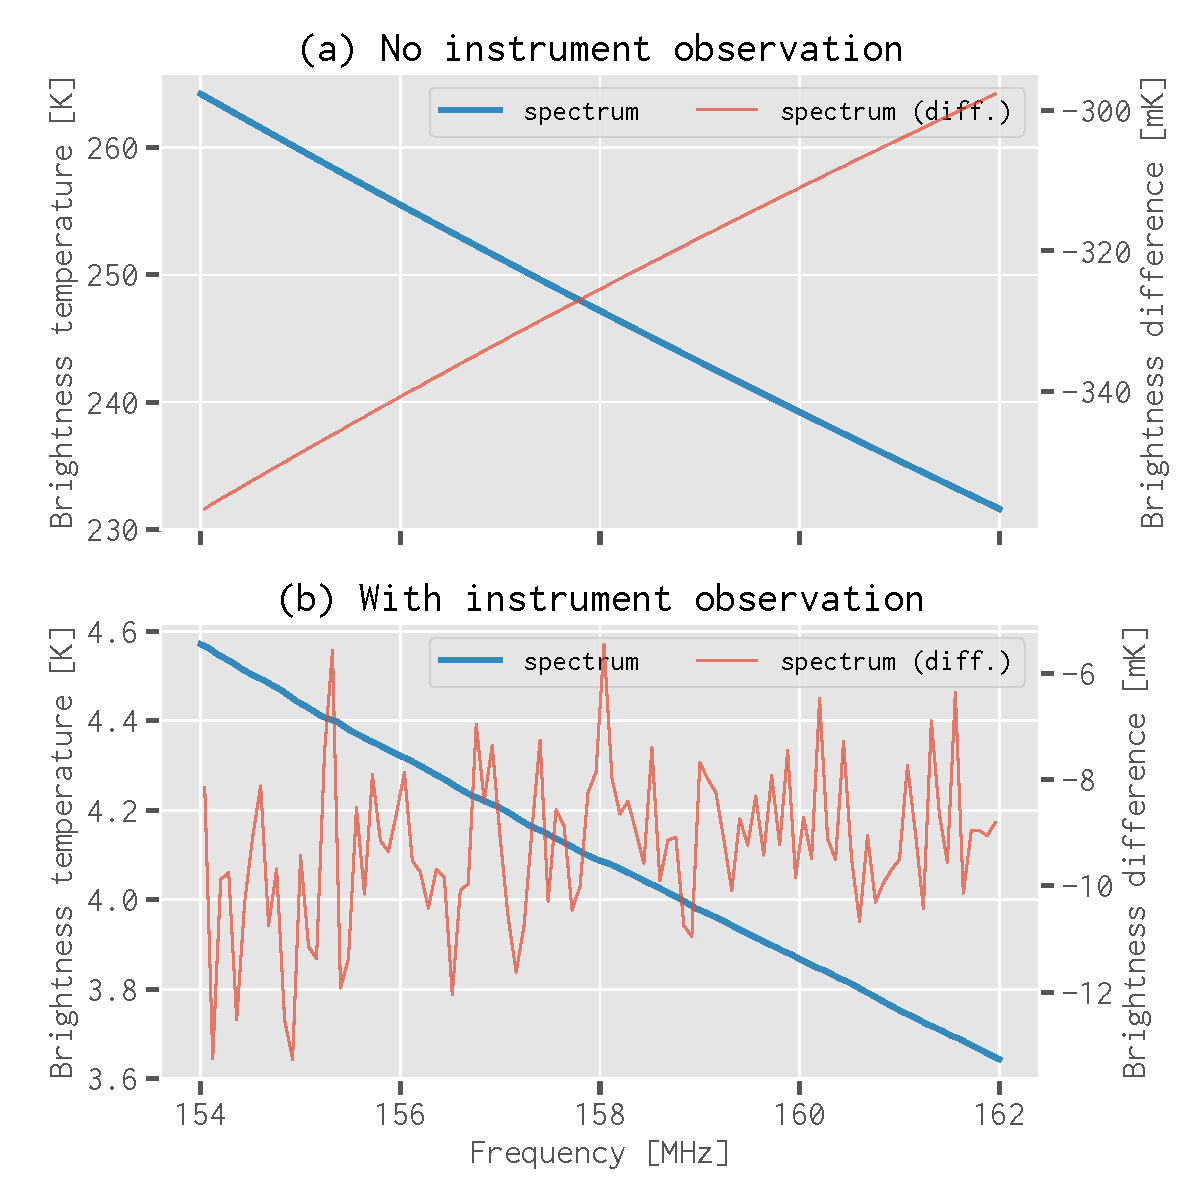
\includegraphics[width=\myfigwidth]{simudata}
  \caption{\label{fig:simudata}%
    Example spectra (the bold blue lines) and the corresponding
    differential spectra (the thin red lines) for the foreground
    emission.
    The top and bottom panels show the cases without and with
    instrument observation, respectively.
  }
\end{figure}


%%----------------------------------------------------------------------
\subsection{Data preprocessing}
\label{sec:preprocessing}

The dataset $S = \{(\B{x}, \,\B{x}_{\R{EoR}})\}$ for the CDAE is derived
from the simulated image cubes $C_{\R{EoR}}$ and $C_{\R{fg}}$, each data
point $(\B{x} = \B{x}_{\R{EoR}} + \B{x}_{\R{fg}}, \,\B{x}_{\R{EoR}})$
representing the total emission and the EoR signal of one sky pixel,
respectively.
The dataset thus consists of $N = \num{360x360} = \num{129600}$ data points.

For the input data $X = \{\B{x}\}$, we propose to apply the
Fourier Transform (FT) along the frequency dimension,
which makes the EoR signal more distinguishable from the
foreground emission and thus easier to be learned by the CDAE
(a comparison with the results derived without applying the FT is
presented in \autoref{sec:why-ft}).
The Blackman-Nuttall window function is applied to suppress the
FT side-lobes caused by the sharp discontinuities at both ends
of the finite frequency band \citep[e.g.,][]{chapman2016}.
It is sufficient to keep only half the Fourier coefficients because
$\B{x}$ is real, thus $\B{x}$ of length $n_f = 101$ is transformed to
be 51 complex Fourier coefficients, among which the $n_{\R{ex}}$
coefficients of the lowest Fourier frequencies are excised since they
are mostly contributed by the spectral-smooth foreground emission.
We adopt $n_{\R{ex}} = 6$ to achieve a balance between the foreground
suppression and the loss of the EoR signal.
The real and imaginary parts of the remaining 45 complex coefficients
are then concatenated into a new real vector of length 90, since the CDAE
requires real data.
Finally, the data are zero-centred and normalised to have unit variance.

The preprocessing steps for the input EoR signal
$X_{\R{EoR}} = \{\B{x}_{\R{EoR}}\}$
are basically the same except for minor adjustments.
After applying the FT, excising the $n_{\R{ex}}$ lowest Fourier
components, and concatenating the real and imaginary parts,
the data elements that have a value less than the 1$^{\R{st}}$
percentile or greater than the 99$^{\R{th}}$ percentile are truncated,
in order to prevent the possible outliers hindering the training of
the CDAE.
Finally, the value range of the data is scaled to be $[-1, 1]$ by
dividing by the maximum absolute value,
which allows to use the `tanh' activation function whose value range
is also $[-1, 1]$ in the output layer of the CDAE
(\autoref{sec:architecture}).


%%----------------------------------------------------------------------
\subsection{Training and results}
\label{sec:training}

The preprocessed dataset is randomly partitioned into
the training set ($S_{\R{tr}}$; 60 per cent) to fit the weights of
filters by minimizing the loss $L$,
the validation set ($S_{\R{val}}$; 20 per cent) to determine the
hyperparameters (e.g., the number of layers and filters, the choice of
loss function),
and the test set ($S_{\R{test}}$; 20 per cent) that is employed to
evaluate the performance of the trained CDAE.

We implement the proposed CDAE using the popular \textsc{Keras}\footnote{%
  Keras: \url{https://keras.io} (version 2.2.0)}
framework \citep{keras} with the \textsc{TensorFlow}\footnote{%
TensorFlow: \url{https://www.tensorflow.org} (version 1.4.1)}
back end \citep{tensorflow}.
The parameters of the Adam optimisation method are set to the default
values (learning rate $\alpha = 0.001$, exponential decay rates for the
first moment estimates $\beta_1 = 0.9$ and for the second moment
estimates $\beta_2 = 0.999$; \citealt{kingma2015}).
The CDAE is trained on the training set ($S_{\R{tr}}$) with a batch size
of 100 for 100 epochs until the training loss converges.

The training and validation losses together with the evaluation index
(i.e., the correlation coefficient $\rho$) calculated on the validation set
($S_{\R{val}}$) during the training phase are shown in \autoref{fig:train}.
The steadily decreasing losses and increasing correlation coefficient
suggest that the CDAE is well trained without overfitting.
The evaluation on the test set ($S_{\R{test}}$) demonstrates that the
trained CDAE achieves excellent performance with a correlation
coefficient of $\rho_{\R{CDAE}} = \num{0.969 +- 0.020}$.
As an example, \autoref{fig:result} illustrates the reconstructed EoR
signal ($\rho = 0.965$) for one random pixel.
In addition, we calculate the one-dimensional power spectra for each
pixel in $S_{\R{test}}$ \citep[e.g.,][]{chapman2013}
and find that the reconstructed EoR signal can recover the total power
to a fraction of $R_{\R{CDAE}} = \num{90.1 +- 8.9}$ per cent.

The achieved excellent performance of the CDAE can be mainly attributed
to the architecture of stacking multiple convolutional layers, which
implements a powerful feature extraction technique by hierarchically
combining the basic features learned in each layer to build more and
more sophisticated features \citep{lecun2015}.
Combined with the flexibility provided by the \num{54337} trainable
weights, the CDAE, after being well trained, can intelligently learn a
model that is optimised to accurately separate the faint EoR signal
\citep[e.g.,][]{domingos2012}.

\begin{figure}
  \centering
  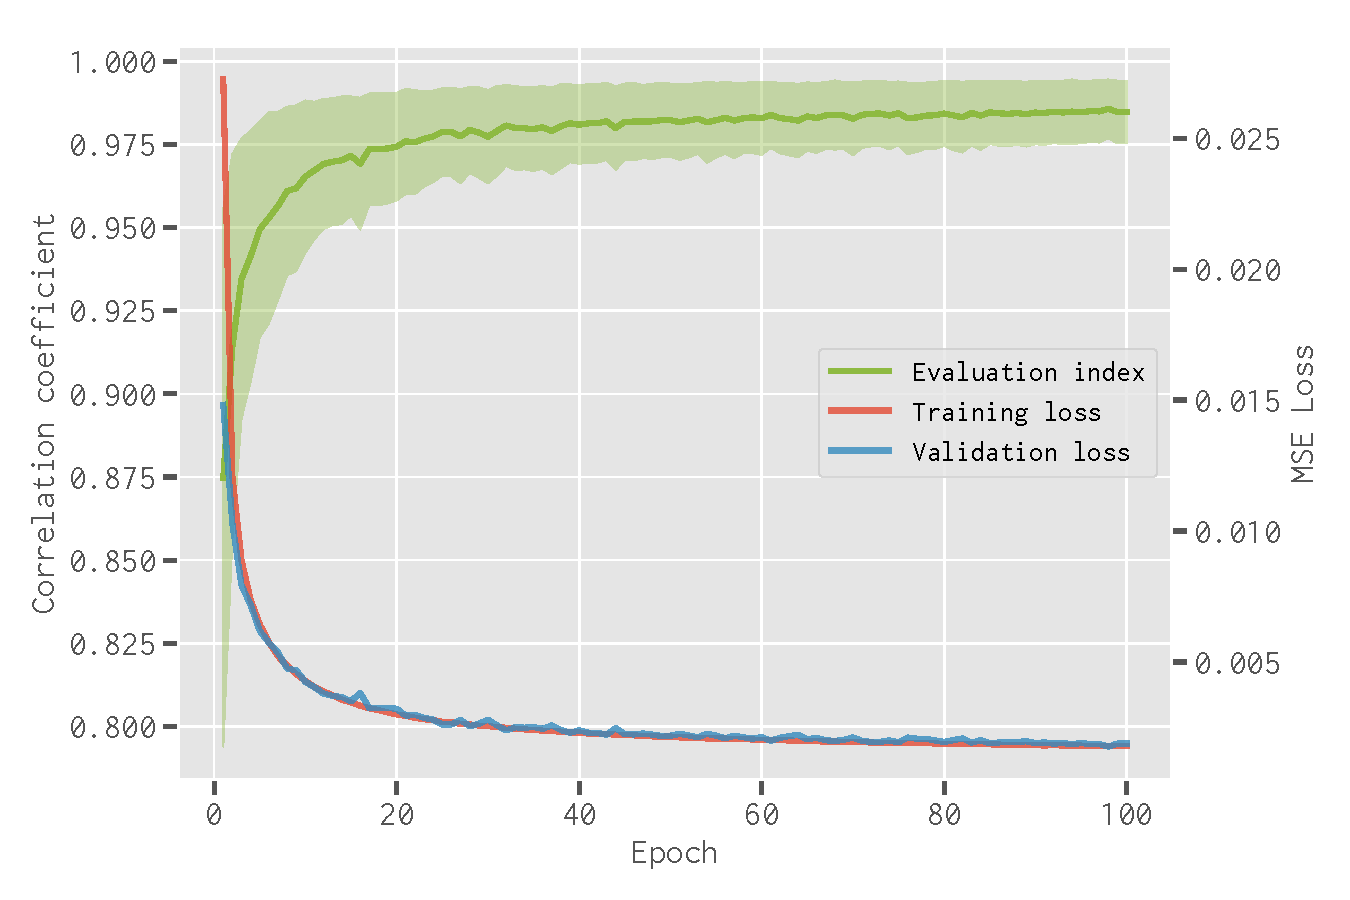
\includegraphics[width=\myfigwidth]{cdae-train}
  \caption{\label{fig:train}%
    The training loss (the red line), validation loss (the blue line),
    and correlation coefficient ($\rho$) calculated on the validation
    set $S_{\R{val}}$ (the green line with the shaded region representing
    the standard deviation) along the training of the CDAE.
  }
\end{figure}

\begin{figure}
  \centering
  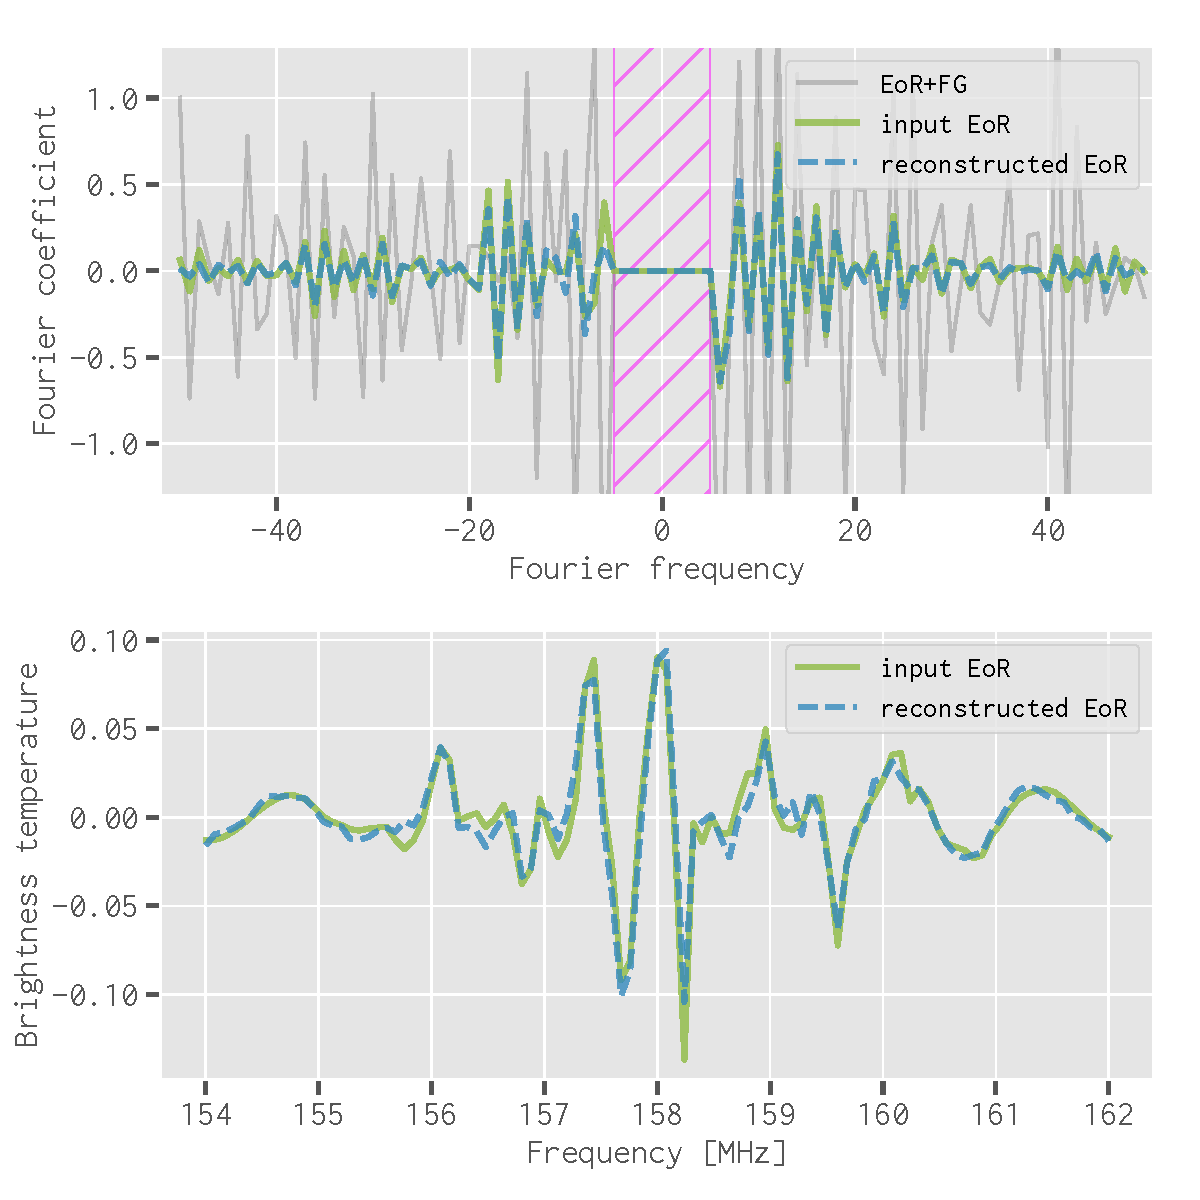
\includegraphics[width=\myfigwidth]{eor-result}
  \caption{\label{fig:result}%
    An example of the EoR signal reconstructed by the trained CDAE for
    one random pixel.
    \textbf{(top)} The input EoR signal $\B{x}_{\R{EoR}}$ (the solid
    green line) and the reconstructed EoR signal $\B{r}_{\R{EoR}}$
    (the dashed blue line) in the Fourier domain.
    The grey line represents the input total emission
    $\B{x} = \B{x}_{\R{fg}} + \B{x}_{\R{EoR}}$.
    The magenta hatched region marks the excised Fourier coefficients
    in data preprocessing.
    \textbf{(bottom)} The input EoR signal $\B{x}_{\R{EoR}}$ (the solid
    green line) and the reconstructed EoR signal $\B{r}_{\R{EoR}}$
    (the dashed blue line) transformed back to the observing frequency
    domain.
  }
\end{figure}


%%======================================================================
\section{Discussions}
\label{sec:discussions}

%%----------------------------------------------------------------------
\subsection{Why preprocess the dataset with Fourier Transform?}
\label{sec:why-ft}

We have performed another experiment using the same CDAE architecture,
dataset, and data preprocessing steps, except for applying the FT
as depicted in \autoref{sec:preprocessing}.
After training the CDAE in the same way as described in
\autoref{sec:training}, the achieved performance is
$\rho_{\R{noFT}} = \num{0.927 +- 0.051}$, which is smaller and has a
larger uncertainty than the case with FT applied, indicating a worse
performance.
We also find that the training process is slightly unstable given the
small spikes on the curves of both the training loss and the correlation
coefficient, and the training loss converges more slowly,
as presented in \autoref{fig:train-noft}.
These indicate that it is beneficial to preprocess the
dataset by applying the FT along the frequency dimension, because the
EoR signal and the foreground emission become more distinguishable
in the Fourier domain, where the fluctuating EoR signal concentrates on
larger Fourier modes while the spectral-smooth foreground emission
distributes mainly on smaller Fourier modes \citep[e.g.,][]{parsons2012}.

\begin{figure}
  \centering
  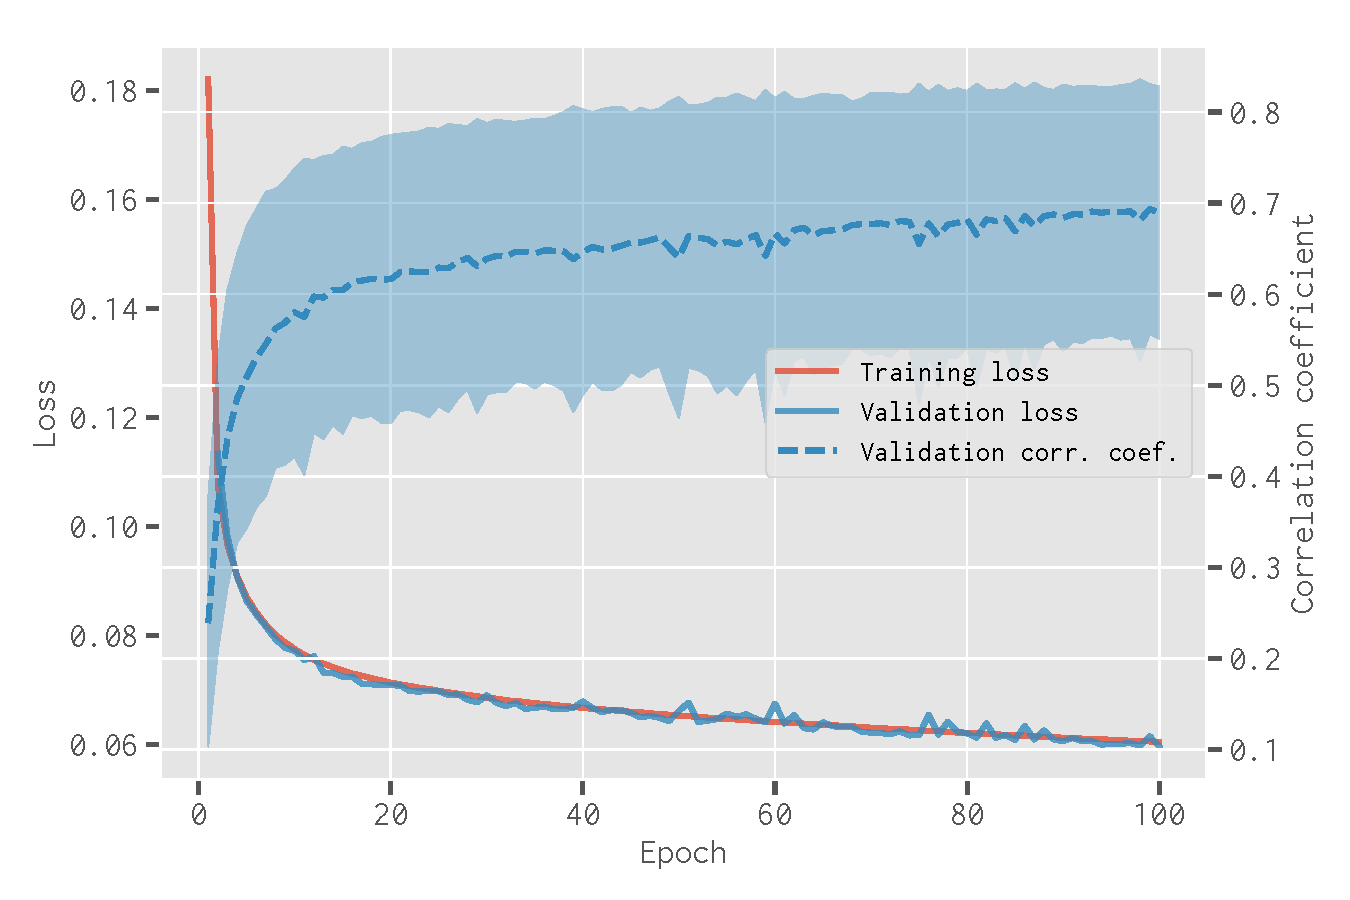
\includegraphics[width=\myfigwidth]{cdae-train-noft}
  \caption{\label{fig:train-noft}%
    Same as \autoref{fig:train} but for the case that the data are
    preprocessed without applying the FT.
  }
\end{figure}


%%----------------------------------------------------------------------
\subsection{Comparing to the polynomial fitting method}
\label{sec:polyfit}

In order to further demonstrate the performance of our method, we have
carried out a comparison between our method and the traditional polynomial
fitting method \citep[e.g.,][]{wang2006,liu2009ps}.
Using the same image cubes simulated in \autoref{sec:simulation},
a low-degree polynomial is fitted along the frequency dimension for each
sky pixel in the image cube of the total emission (i.e.,
$C_{\R{tot}} = C_{\R{EoR}} + C_{\R{fg}}$).
Then by subtracting the fitted smooth component, which is regarded as
the foreground emission, the EoR signal is expected to be uncovered.
We have tested polynomials of the degree from 2 (quadratic) to
5 (quintic), and find that the quartic polynomial (degree of 4)
can give the best result.
However, the correlation coefficient calculated for the separated EoR
signal in such a case is only $\rho_{\R{poly}} = \num{0.241 +- 0.103}$,
which indicates that the polynomial fitting method
performs poorly in removing the foreground emission.
As illustrated in \autoref{fig:simudata}(b), the frequency-dependent
beam effects cause significant fluctuations, which can be even stronger
than the EoR signal, on the originally smooth foreground spectra.
The polynomial fitting method, which can only model the smooth
spectrum, is unable to distinguish these rapid fluctuations from the
EoR signal, hence leading to inferior results.
On the contrary, given its flexibility and data-driven nature,
the CDAE can distil knowledge from the data to optimise itself for
the EoR signal separation and hence achieve superior performance.


%%======================================================================
\section{Summary}
\label{sec:summary}

The frequency-dependent beam effects of interferometers can cause
rapid fluctuations along the frequency dimension,
which destroy the smoothness of the foreground spectra and prevent
traditional foreground removal methods from uncovering the EoR signal.
Given the difficulties in crafting practicable models to overcome the
complicated beam effects, methods that can intelligently learn tailored
models from the data seem more feasible and appealing.
To this end, we have proposed a deep-learning-based method that uses
a 9-layer CDAE to separate the EoR signal.
The CDAE has been trained on the simulated SKA images and has achieved
excellent performance.
We conclude that the CDAE has outstanding ability to overcome the
complicated beam effects and accurately separate the faint EoR signal,
exhibiting the great potential of deep-learning-based methods
to play an important role in the forthcoming EoR experiments.


%%======================================================================
\section*{Acknowledgements}

We would like to thank Jeffrey Hsu for reading the manuscript and
providing suggestions.
This work is supported by
the Ministry of Science and Technology of China
(grant Nos. 2018YFA0404601, 2017YFF0210903),
and the National Natural Science Foundation of China
(grant Nos. 11433002, 11621303, 11835009, 61371147).


%%======================================================================
%% References

\bibliographystyle{mnras}
\bibliography{references}


%%======================================================================
%% Appendix

% \appendix


%%======================================================================
% Don't change these lines
\bsp	% typesetting comment
\label{lastpage}
\end{document}

%% EOF
